\documentclass[12pt,a4paper]{article}
\usepackage[utf8]{inputenc}
\usepackage[T1]{fontenc}
\usepackage{lmodern}
\usepackage[margin=1in]{geometry}
\usepackage{xcolor}
\usepackage{tcolorbox}
\usepackage{enumitem}
\usepackage{hyperref}
\usepackage{babel}
\usepackage{graphicx}
\usepackage{url}
\usepackage{amsmath}
\usepackage{pgfplots}
\pgfplotsset{compat=1.17}
\usepackage{amsmath}
\usepackage{hyperref}
\usepackage{fontawesome}
\usepackage{float}    % For enforcing image position with [H]

% Define colors
\definecolor{sectioncolor}{RGB}{0,102,204}
\definecolor{subsectioncolor}{RGB}{0,153,76}
\definecolor{boxcolor}{RGB}{240,248,255}

% Define styles for sections and subsections
\newcommand{\colorsection}[1]{{\color{sectioncolor}\Large\bfseries#1}}
\newcommand{\colorsubsection}[1]{{\color{subsectioncolor}\large\bfseries#1}}

\title{\textbf{Phase 2 - Report for DFN-PSAN Project}}
\author{
    Ayush Kumar Mishra (12240340), Ayush Patel (12240350) \\ % First line with two authors
    Divyanshu Prakash (12240540), Shivam (12241710), Ujjwal Raj (12241920) % Second line with three authors
}
\date{}
\begin{document}
\maketitle

\begin{center}
    \section*{\textcolor{teal}{\huge{Krishi.ai \href{https://krishi-ai.onrender.com/}{\faExternalLink}}}}
    \section*{\textcolor{teal}{\large{Repo \href{https://github.com/shivamlth27/Krishi_ai}{\faExternalLink}}}}
\end{center}

\section*{\colorsection{1. Project Directory}}
\begin{figure}[H] % [H] forces the figure to stay here, exactly where it is in the document
    \centering
    \fbox{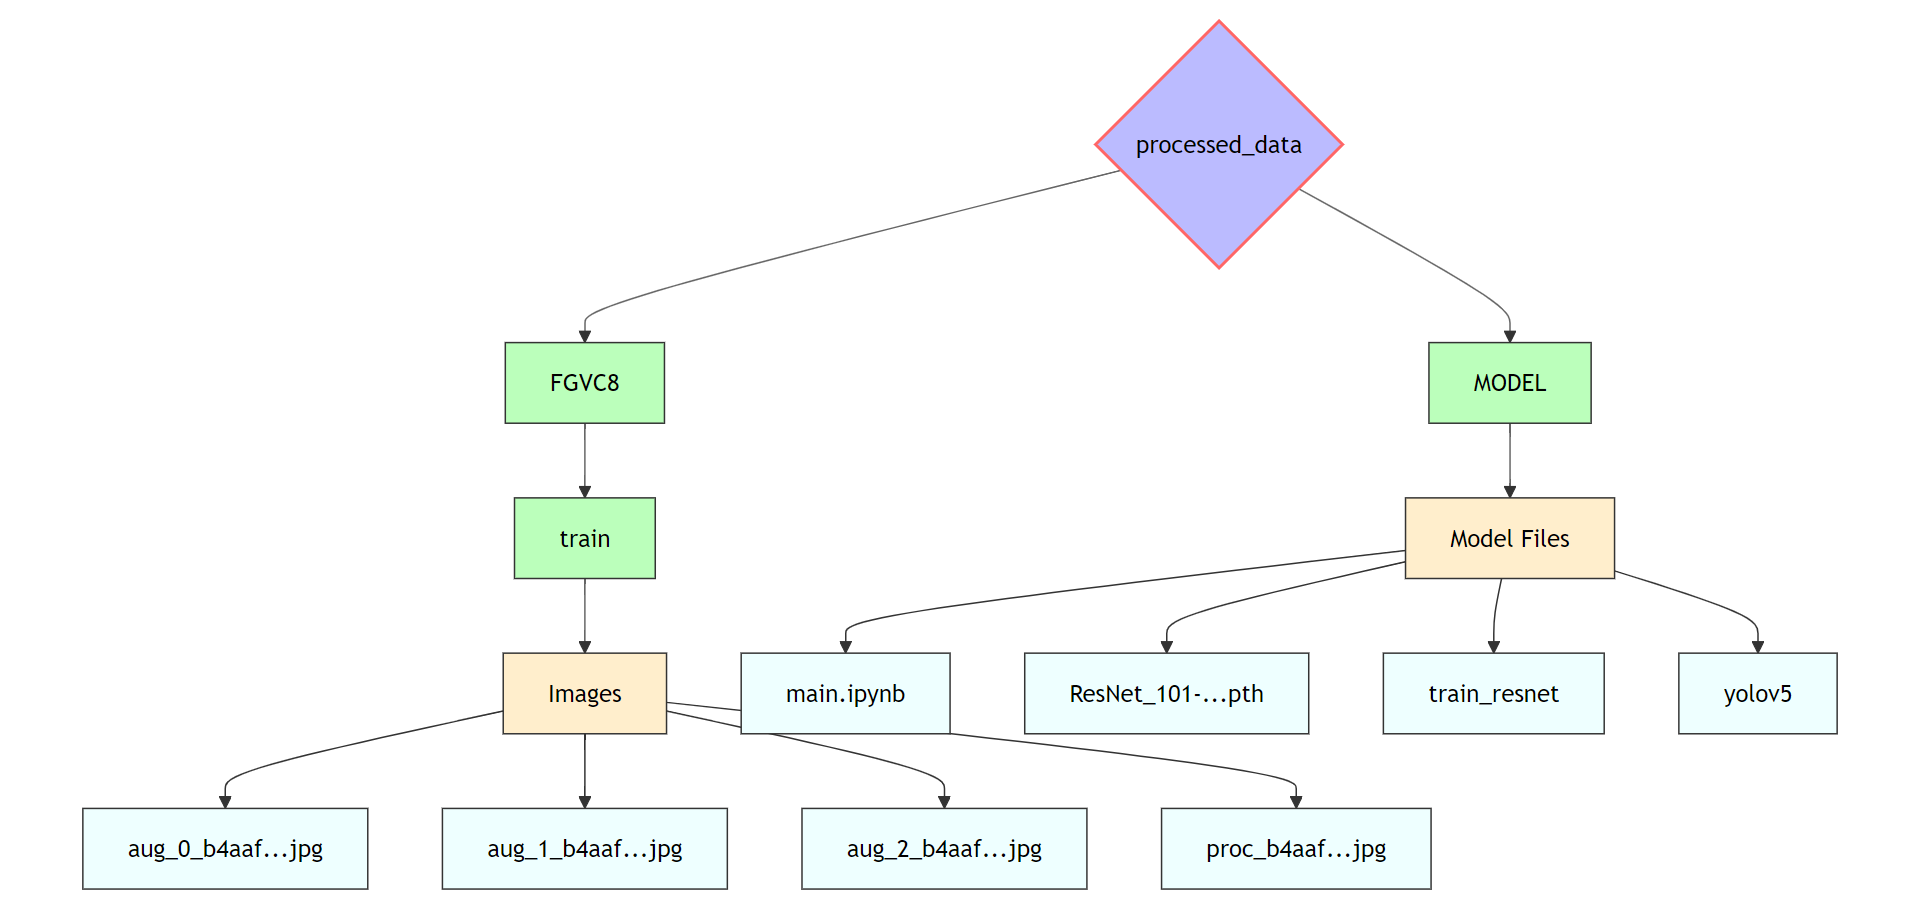
\includegraphics[width=0.7\textwidth]{image6(flowchart1).png}} % Increased size of the first image
    \caption{Flowchart 1 for data directory.}
\end{figure}
\begin{figure}[H] % [H] forces the figure to stay here, exactly where it is in the document
    \centering
    \fbox{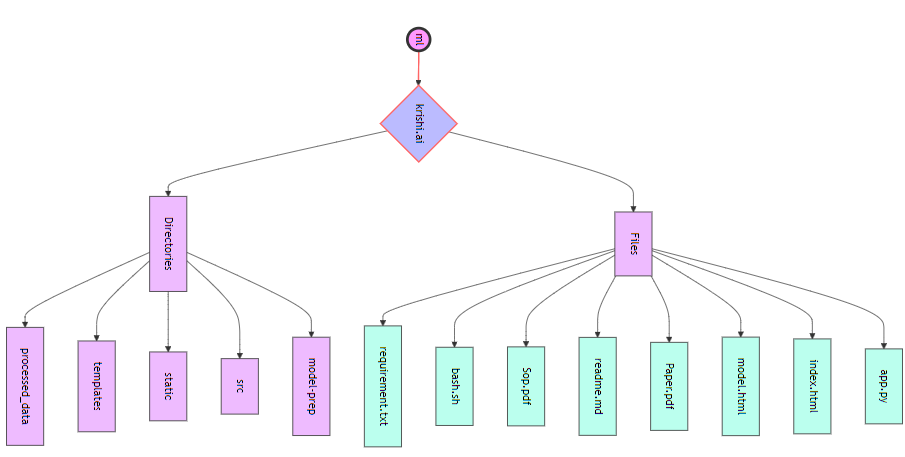
\includegraphics[width=0.7\textwidth]{image7(flowchart2).png}} % Increased size of the first image
    \caption{Flowchart 2 for Project directory.}
\end{figure}
% \begin{figure}[H] % [H] forces the figure to stay here, exactly where it is in the document
%     \centering
%     \fbox{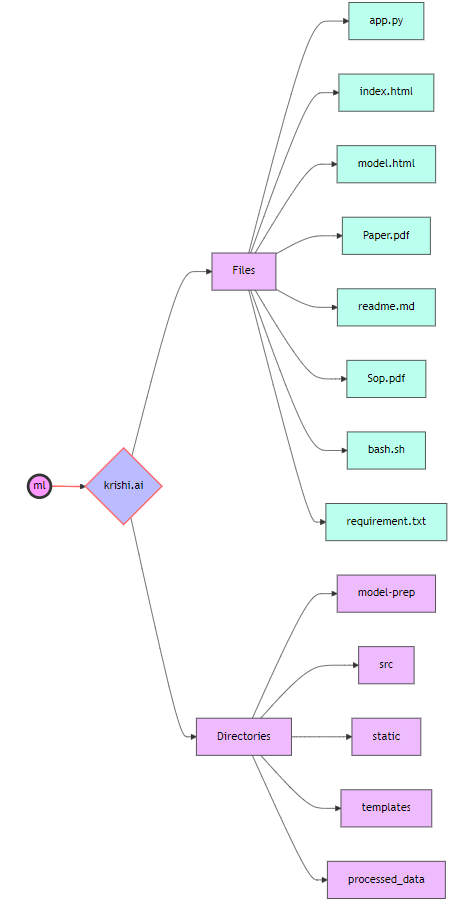
\includegraphics[width=0.5\textwidth]{1.png}} % Increased size of the first image
%     \caption{Flowchart 2 for Project directory.}
% \end{figure}
\section*{\colorsection{2. Project Workflow}}
\section*{\colorsection{3. Achievements accomplished in this phase.}}
\subsection*{Website Part:}
\subsubsection*{Home interface.}
\subsubsection*{Loading Image}

\subsection*{Model Part:}


\subsubsection*{1 Loading our required data set.}
\subsubsection*{2 Dividing the data for training and validation purposes. }
\subsubsection*{3 Preprocessing the image .}


\begin{figure}[H] % [H] forces the figure to stay here, exactly where it is in the document
    \centering
    \fbox{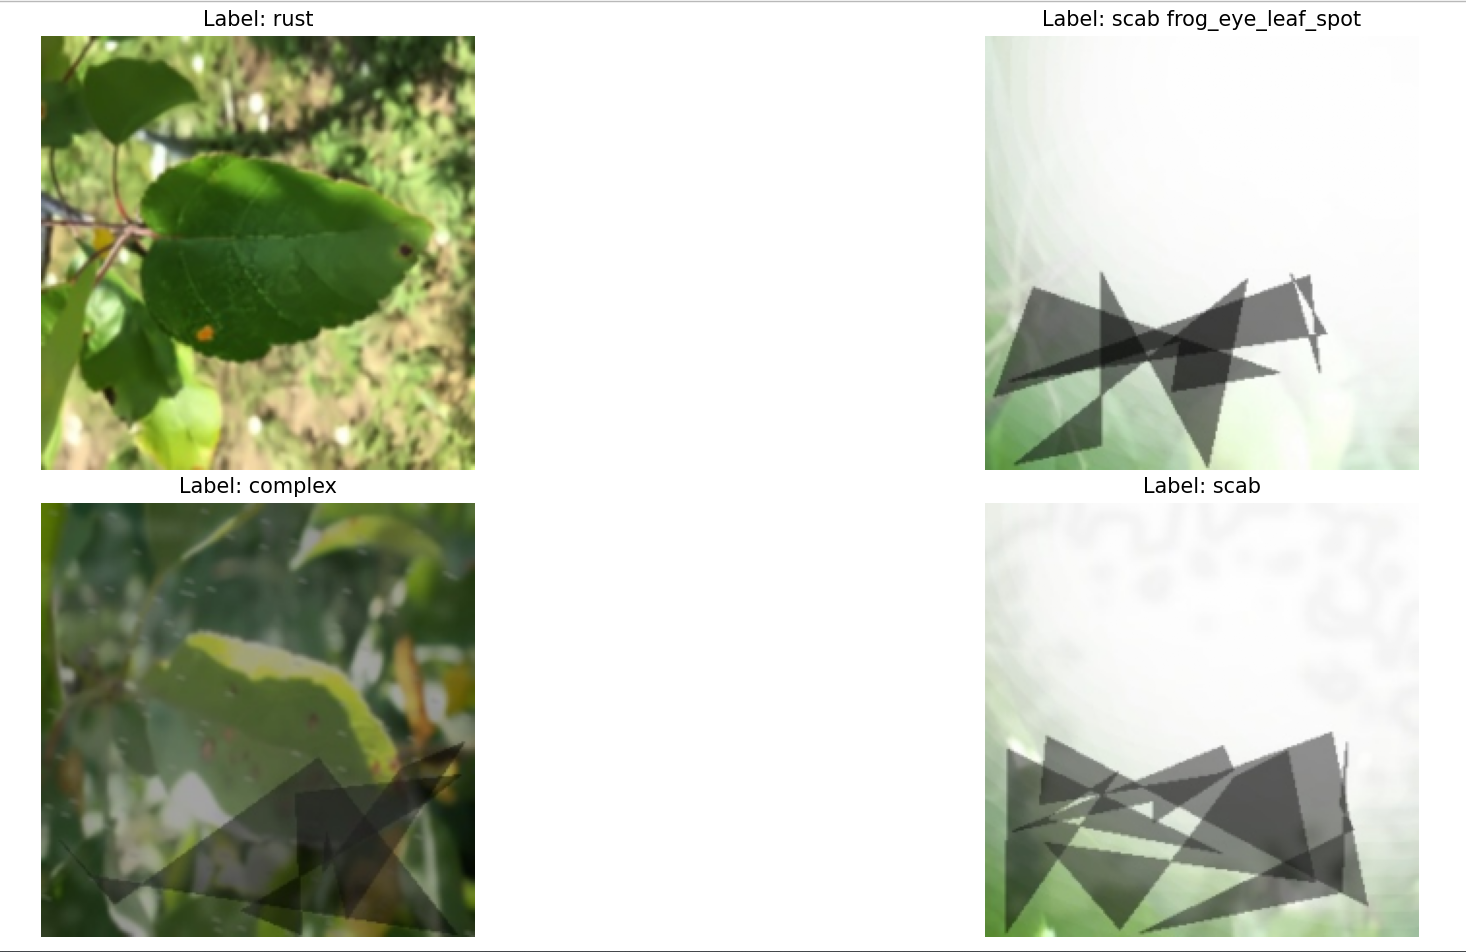
\includegraphics[width=0.7\textwidth]{image1.png}} % Increased size of the first image
    \caption{This is an example image with fixed position.}
\end{figure}

\begin{figure}[H] % [H] forces the figure to stay here, exactly where it is in the document
    \centering
    \fbox{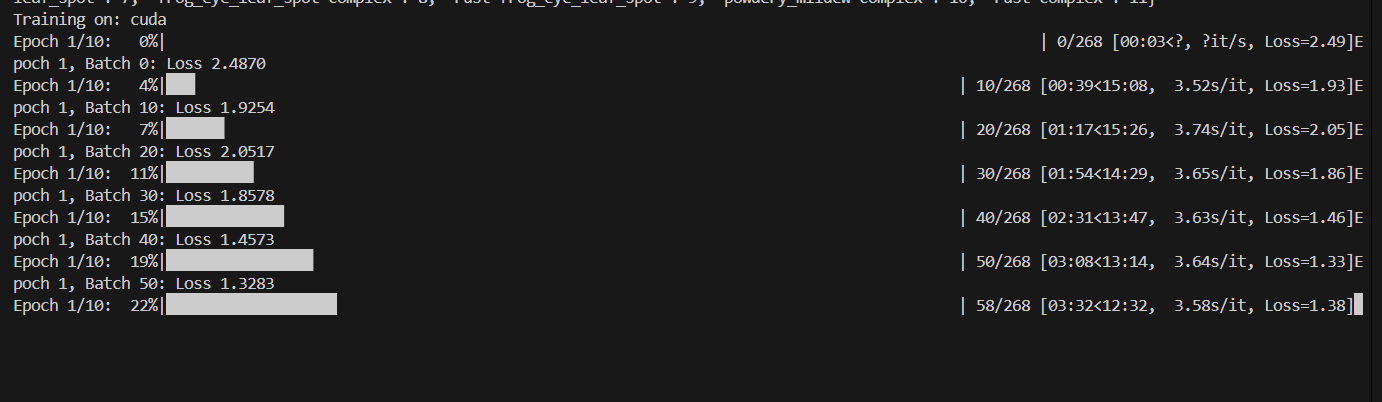
\includegraphics[width=0.7\textwidth]{image2.png}} % Increased size of the second image
    \caption{This is an example image with fixed position.}
\end{figure}

\begin{figure}[H] % [H] forces the figure to stay here, exactly where it is in the document
    \centering
    \fbox{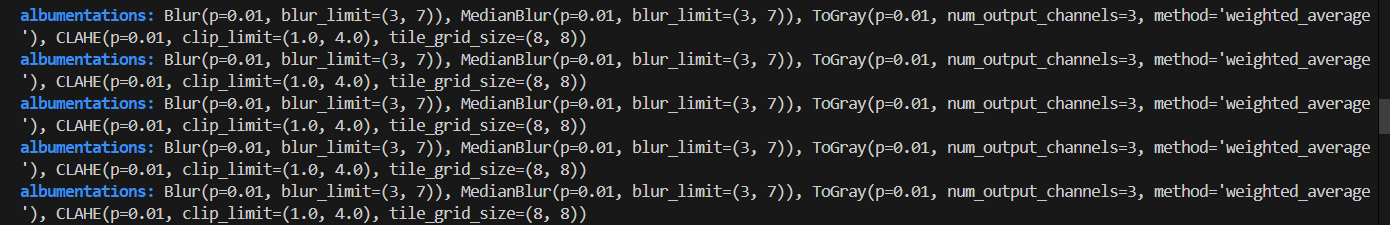
\includegraphics[width=0.7\textwidth]{image3.png}} % Increased size of the third image
    \caption{This is an example image with fixed position.}
\end{figure}

\begin{figure}[H]
    \centering
    \begin{minipage}{0.45\textwidth}
        \centering
        \fbox{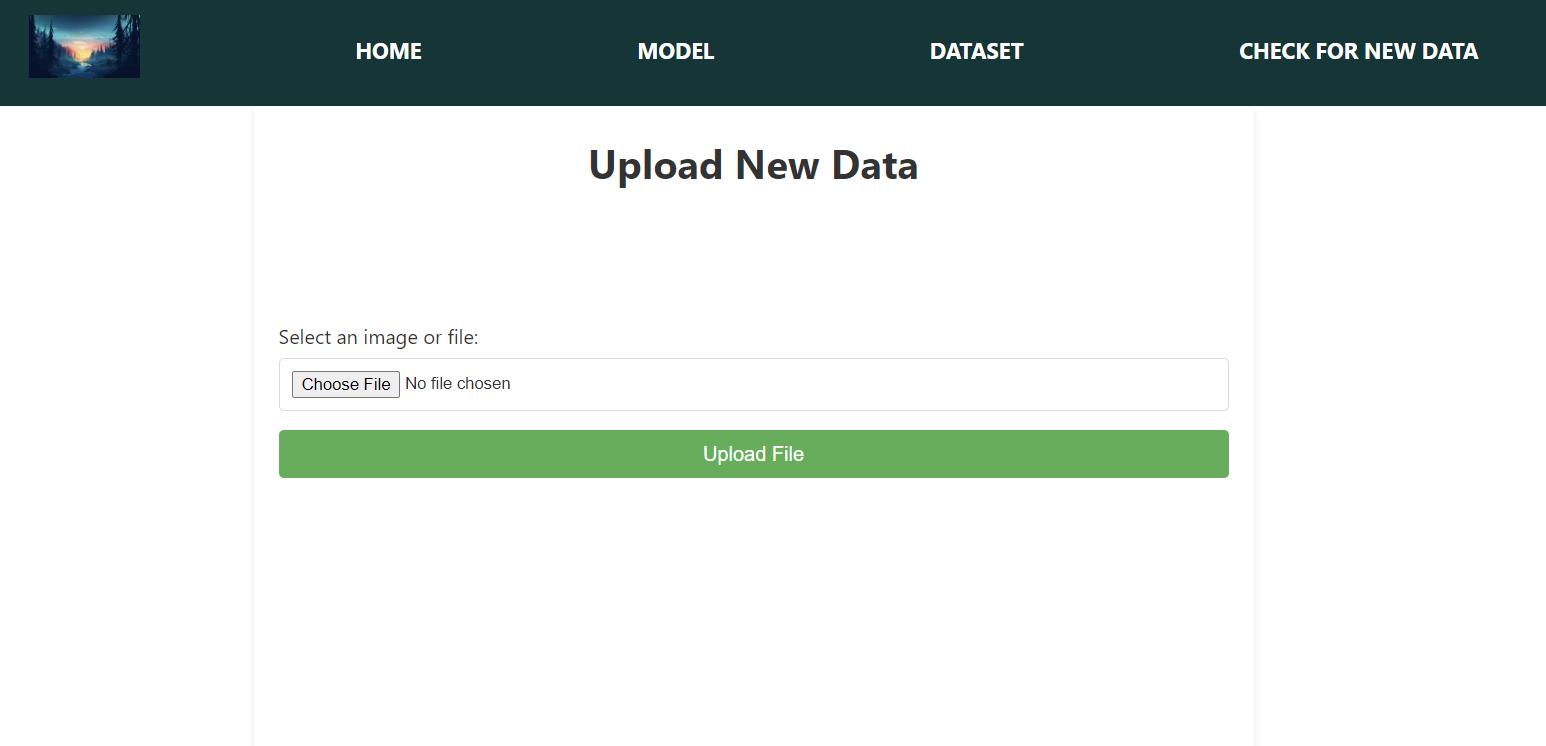
\includegraphics[width=\textwidth]{image4.png}} % Increased size of the first image
        \caption{First image}
    \end{minipage}
    \hspace{0.05\textwidth} % Space between the images
    \begin{minipage}{0.45\textwidth}
        \centering
        \fbox{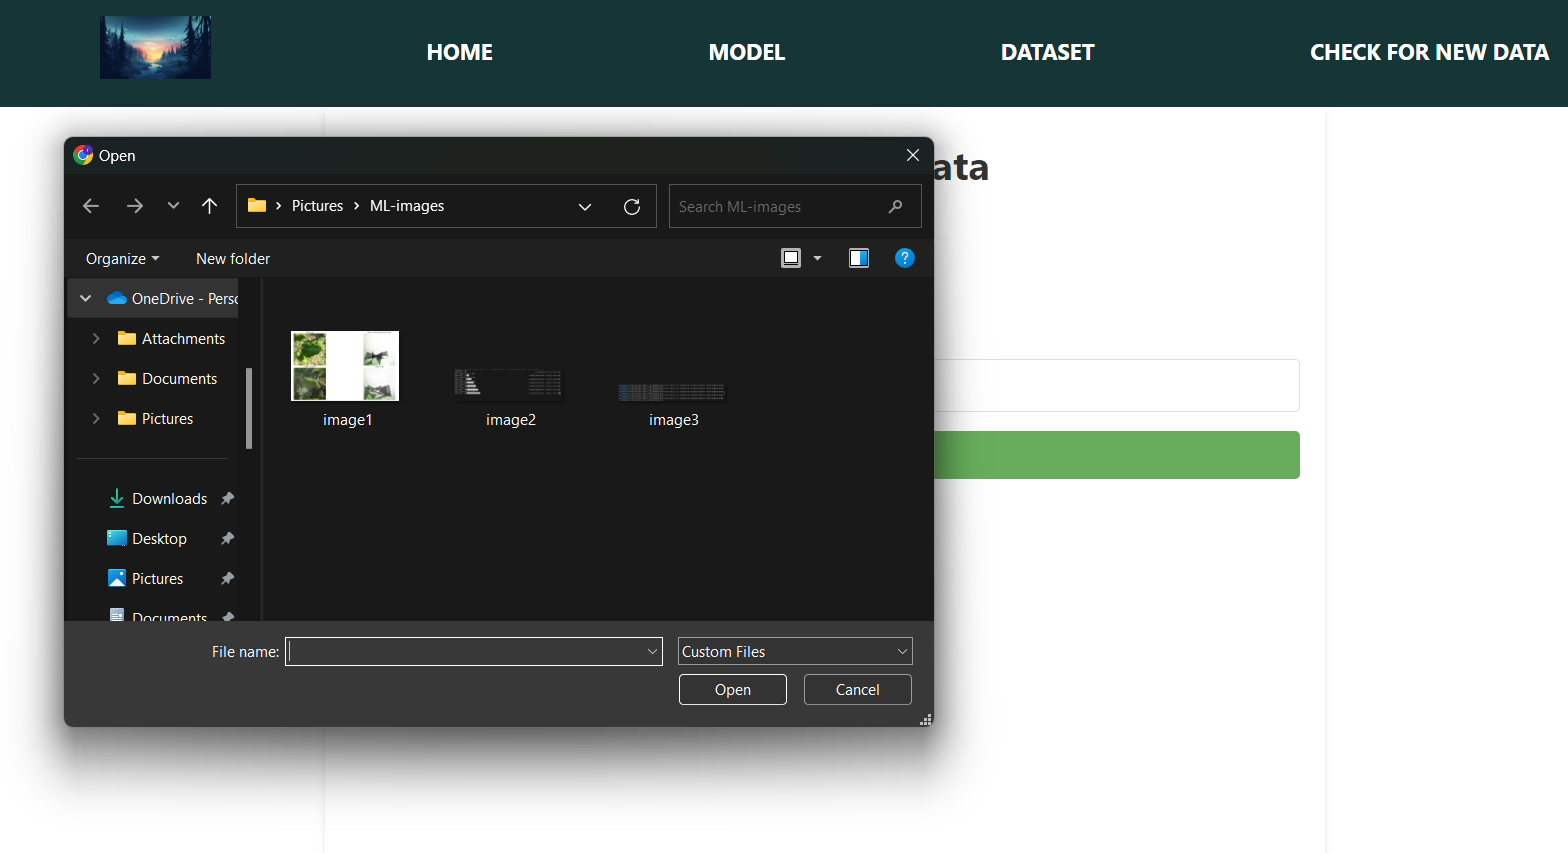
\includegraphics[width=\textwidth]{image5.png}} % Increased size of the second image
        \caption{Second image}
    \end{minipage}
\end{figure}
\section*{\colorsection{4.Tasks to be done}}
\section*{\colorsection{5.Members Contribution}}
\begin{tcolorbox}[colback=blue!5!white, colframe=blue!75!black, title=Ayush Patel (12240350)]
    \textcolor{blue}{\textbf{Data Collection \& Preprocessing:}} Ayush Patel was responsible for collecting the required datasets and ensuring the quality of the data by performing various preprocessing steps. He handled image resizing, noise reduction, and augmentation tasks, ensuring that the data was properly prepared for training.
    
    \vspace{0.2cm}
    
    \textcolor{blue}{\textbf{Data Management:}} He also managed the dataset versioning and ensured smooth data handling for training and validation.
\end{tcolorbox}

\vspace{0.5cm}

\begin{tcolorbox}[colback=green!5!white, colframe=green!75!black, title=Ayush Kumar Mishra (12240340)]
    \textcolor{green}{\textbf{Model Architecture Implementation (DFN):}} Ayush played a key role in implementing the Deep Fusion Network (DFN) backbone using the YOLOv5 architecture. He designed and integrated the multi-level feature fusion module, ensuring efficient feature extraction for the classification task.
    
    \vspace{0.2cm}
    
    \textcolor{green}{\textbf{Code Optimization:}} He optimized the model for better computational efficiency and reduced training time.
\end{tcolorbox}

\vspace{0.5cm}

\begin{tcolorbox}[colback=red!5!white, colframe=red!75!black, title=Divyanshu Prakash (12240540)]
    \textcolor{red}{\textbf{Pyramid Squeezed Attention Module (PSA):}} Divyanshu contributed to the integration of the Pyramid Squeezed Attention Network (PSAN) module. He worked on fine-tuning the attention layers to enhance the model’s feature extraction capabilities.
    
    \vspace{0.2cm}
    
    \textcolor{red}{\textbf{Model Tuning:}} He also focused on hyperparameter tuning, adjusting learning rates, batch sizes, and regularization techniques to achieve better accuracy.
\end{tcolorbox}

\vspace{0.5cm}

\begin{tcolorbox}[colback=orange!5!white, colframe=orange!75!black, title=Shivam (12241710)]
    \textcolor{orange}{\textbf{Project Workflow \& Coordination:}} Shivam was in charge of setting up the overall project workflow, including task assignment and coordination. He ensured that team members were aligned with their roles and that deadlines were met.
    
    \vspace{0.2cm}
    
    \textcolor{orange}{\textbf{Data Splitting \& Model Training:}} He led the effort in dividing the dataset into training and validation sets, ensuring proper distribution and randomization. Shivam also managed the training process, implementing early stopping mechanisms and performance monitoring during the training phase.
\end{tcolorbox}

\vspace{0.5cm}

\begin{tcolorbox}[colback=purple!5!white, colframe=purple!75!black, title=Ujjwal Raj (12241920)]
    \textcolor{purple}{\textbf{Website Development:}} Ujjwal spearheaded the development of the website’s interface. He created the home page, designed the layout, and ensured the loading of images for disease classification on the platform.
    
    \vspace{0.2cm}
    
    \textcolor{purple}{\textbf{Deployment:}} He was responsible for integrating the trained model into the website and setting up the deployment pipeline on the Render platform. Ujjwal ensured that the model predictions were available through a user-friendly interface.
\end{tcolorbox}
\begin{center}
***
\end{center}

\end{document}
